\section{Results}
\label{sec:results}

We report four blocks of results: reasoning length (\secref{sec:results:tokens}), single-turn accuracy and the pooled sweet-spot test (\secref{sec:results:accuracy}), apology onset (\secref{sec:results:apology}), and the two-turn \flipflop carry-over (\secref{sec:results:flipflop}). Per-(model$\times$dataset) heterogeneity is summarised in \secref{sec:results:heterogeneity}.

\subsection{Reasoning length grows with tone intensity}
\label{sec:results:tokens}

Table~\ref{tab:tokens} reports mean completion tokens per (model, dataset, tone). On \tqa the increase from \Lz to the peak (\Lf for both models) is substantial: $+36\%$ for \gptfomini ($165.7\rightarrow 224.9$ tokens) and $+57\%$ for \gptfo ($137.1\rightarrow 215.3$ tokens). Paired Wilcoxon signed-rank tests on per-item token differences $(\Lf-\Lz)$ yield $p=3.32\times 10^{-13}$ on \gptfomini and $p=5.06\times 10^{-9}$ on \gptfo. The Spearman correlation between tone level $0$--$5$ and per-item tokens on \tqa is $\rho=0.30$ ($p<10^{-6}$) for \gptfo and $\rho=0.12$ ($p<10^{-4}$) for \gptfomini.

\begin{table}[h]
\centering
\caption{Mean completion tokens per (model, dataset, tone). Peak cell per row in \textbf{bold}. Token growth is largest on \tqa and concentrates at \Lf (``I'm going to grade this''). \gsm and \mmlu show smaller but consistent positive movement.}
\label{tab:tokens}
\small
\begin{tabular}{@{}llcccccc@{}}
\toprule
\textbf{Model} & \textbf{Dataset} & \Lz & \Lo & \Lt & \Lth & \Lf & \Lfi \\
\midrule
\gptfomini & \tqa  & 165.7 & 197.8 & 198.6 & 194.3 & \textbf{224.9} & 184.3 \\
\gptfo     & \tqa  & 137.1 & 184.7 & 149.4 & 171.4 & \textbf{215.3} & 191.8 \\
\gptfomini & \gsm  & 139.2 & 150.0 & \textbf{153.0} & 149.9 & 148.1 & 149.9 \\
\gptfo     & \gsm  & 153.0 & 162.2 & 160.1 & 154.0 & \textbf{166.0} & 160.5 \\
\gptfomini & \mmlu & 401.1 & \textbf{422.4} & 419.4 & 415.5 & 410.8 & 394.5 \\
\gptfo     & \mmlu & 378.5 & 379.9 & 381.9 & 386.5 & 381.9 & \textbf{408.5} \\
\bottomrule
\end{tabular}
\end{table}

\begin{figure}[h]
\centering
\begin{subfigure}[b]{0.48\textwidth}
    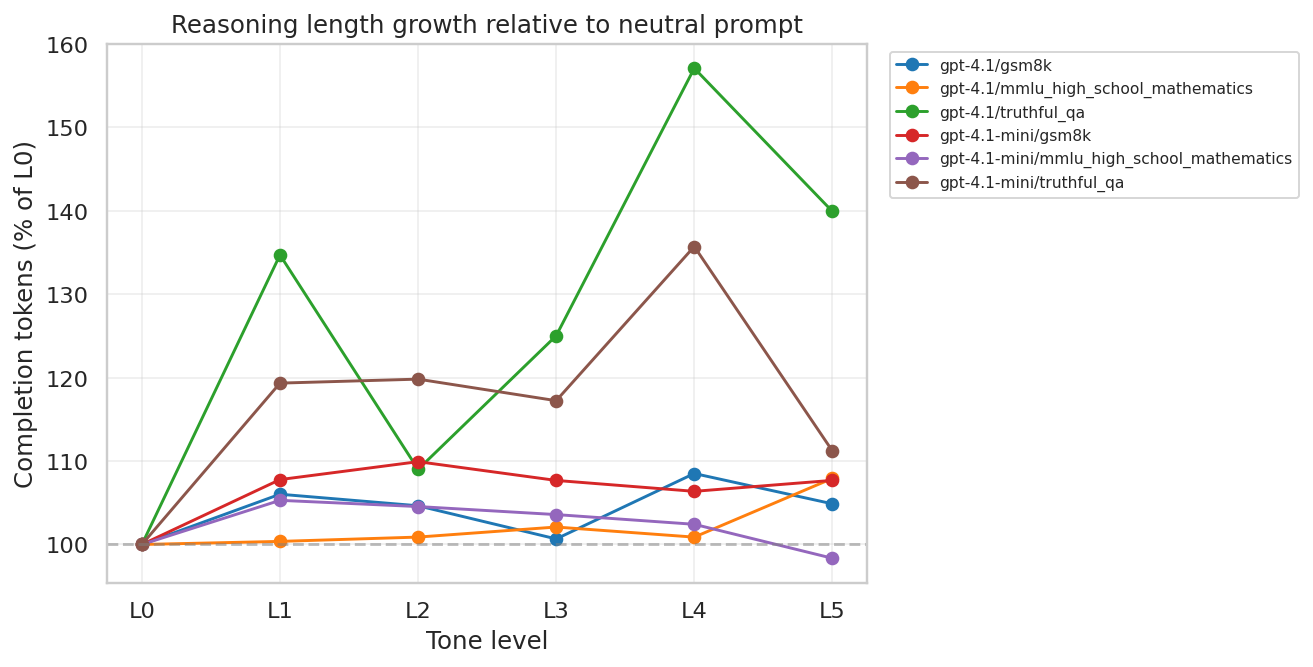
\includegraphics[width=\linewidth]{figures/token_growth.png}
    \caption{Mean completion-token growth relative to neutral, per (model, dataset, tone).}
    \label{fig:token_growth}
\end{subfigure}\hfill
\begin{subfigure}[b]{0.48\textwidth}
    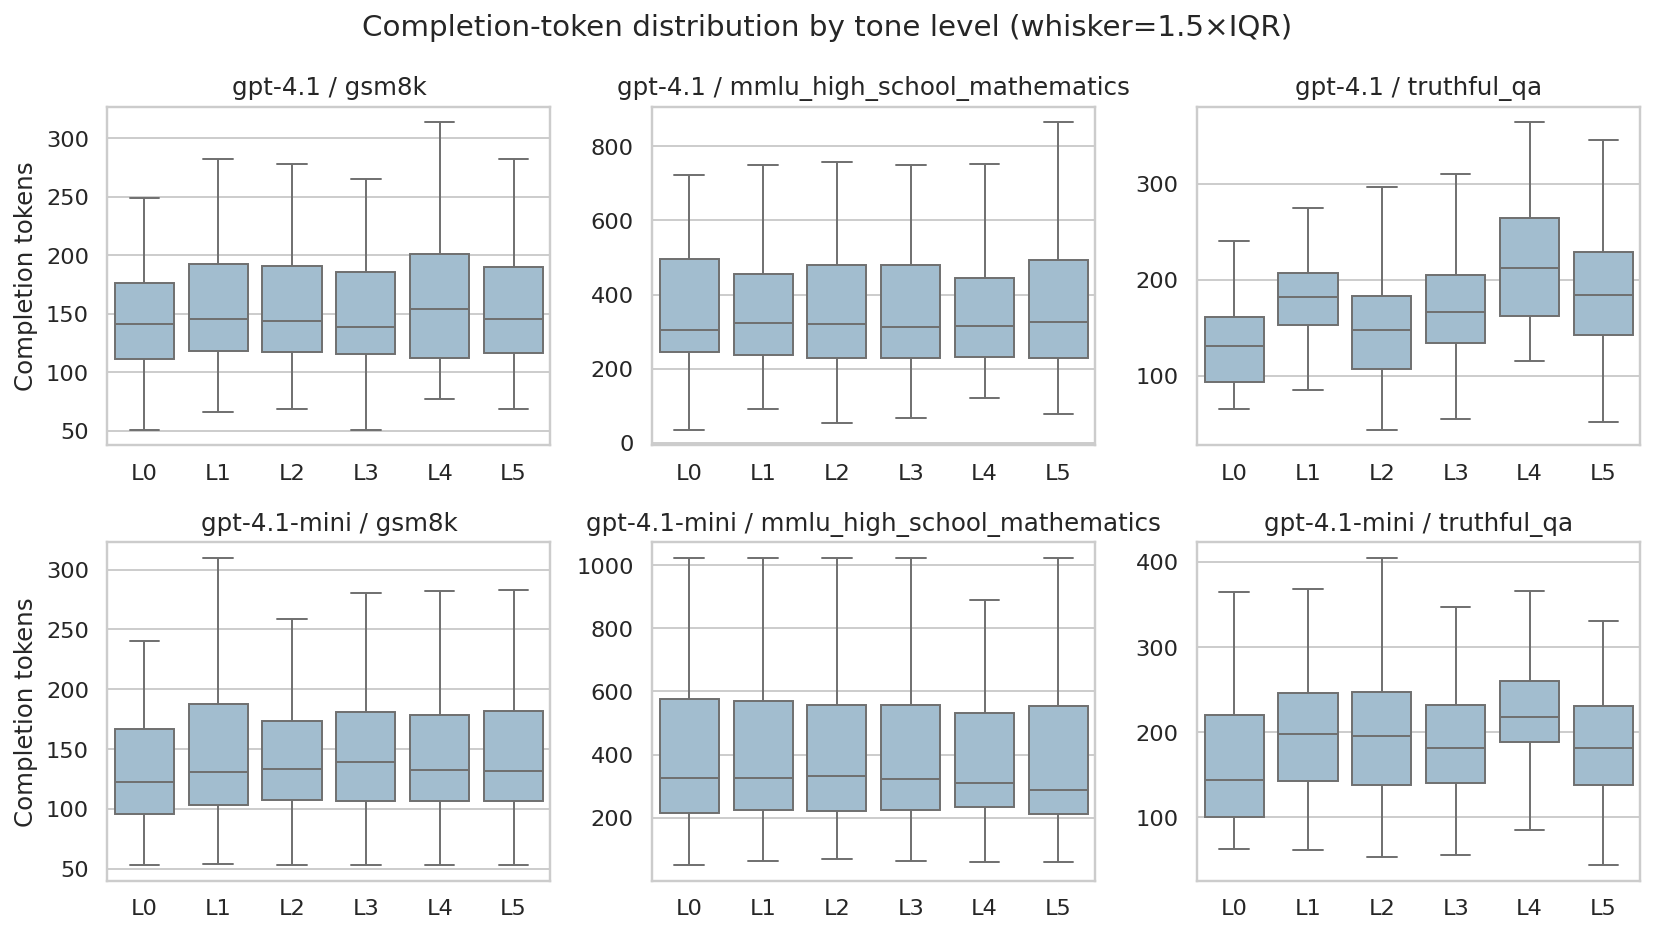
\includegraphics[width=\linewidth]{figures/tokens_box_per_dataset.png}
    \caption{Per-item completion-token distribution by tone, per (model, dataset).}
    \label{fig:tokens_box}
\end{subfigure}
\caption{Reasoning-length response to tone. Token expenditure on \tqa peaks at \Lf for both models. The effect is significant under paired Wilcoxon ($p \le 10^{-9}$) and survives the trend test (Spearman $\rho>0.1$, $p<10^{-4}$).}
\label{fig:tokens}
\end{figure}

Qualitatively, responses also change in structure: under \Lz the model frequently emits a single flowing prose paragraph, while under \Lf it explicitly enumerates each choice and weighs it. The token growth is therefore not pure verbosity but additional structured deliberation.

\subsection{Single-turn accuracy: a small directional sweet spot on TruthfulQA}
\label{sec:results:accuracy}

Table~\ref{tab:accuracy} reports single-turn accuracy across all conditions. Two observations dominate. First, on \tqa both models show a directional benefit from skeptical tones: \gptfomini is monotonically higher under all of \Lo--\Lfi vs.\ \Lz, with a $+3$--$+4$\,pp range, and \gptfo peaks at \Lf ($+4$\,pp). Second, \gsm and \mmlu sit at or near ceiling: accuracy moves by no more than $\pm 2$\,pp across the entire ladder and no clear pattern emerges.

\begin{table}[h]
\centering
\caption{Single-turn accuracy per (model, dataset, tone). Best per row in \textbf{bold}. \tqa is the only dataset with headroom for tone to operate on; \gsm and \mmlu sit near ceiling.}
\label{tab:accuracy}
\small
\begin{tabular}{@{}llcccccc@{}}
\toprule
\textbf{Model} & \textbf{Dataset} & \Lz & \Lo & \Lt & \Lth & \Lf & \Lfi \\
\midrule
\gptfomini & \tqa  & 0.72 & 0.75 & 0.75 & 0.75 & 0.75 & \textbf{0.76} \\
\gptfo     & \tqa  & 0.86 & 0.82 & 0.86 & 0.82 & \textbf{0.90} & 0.86 \\
\gptfomini & \gsm  & \textbf{0.96} & \textbf{0.96} & 0.94 & \textbf{0.96} & 0.94 & 0.95 \\
\gptfo     & \gsm  & \textbf{0.92} & \textbf{0.92} & 0.90 & \textbf{0.92} & 0.90 & \textbf{0.92} \\
\gptfomini & \mmlu & 0.93 & 0.90 & 0.90 & 0.89 & \textbf{0.94} & 0.93 \\
\gptfo     & \mmlu & \textbf{0.98} & \textbf{0.98} & \textbf{0.98} & \textbf{0.98} & 0.96 & 0.96 \\
\bottomrule
\end{tabular}
\end{table}

Per-item McNemar tests on \Lz vs.\ each of \Lo--\Lfi are not significant individually at $p<0.05$, which at the per-cell sample size of $n=100$ (or $50$) is consistent with a true effect of $\sim 3$\,pp. To increase power we pool the five skeptic levels into a per-item majority vote (\Lo--\Lfi) and compare against \Lz on \tqa. Table~\ref{tab:pooled} reports the result. On \gptfomini, every one of the four items on which \Lz and the skeptic majority disagree falls in favour of the skeptic; the one-sided exact binomial $p=0.0625$ ($4$ successes out of $4$). On \gptfo the disagreement is symmetric and not informative at $n=50$.

\begin{table}[h]
\centering
\caption{Pooled skeptic-majority (\Lo--\Lfi) vs.\ neutral (\Lz) accuracy on \tqa, per item. The direction on \gptfomini is clean ($4$/$4$ disagreements favour the skeptic), and the one-sided exact binomial is at the floor at $n=4$.}
\label{tab:pooled}
\small
\begin{tabular}{@{}lccccccc@{}}
\toprule
\textbf{Model} & $n$ & \Lz\textbf{ acc} & \textbf{skeptic-maj acc} & $\Delta$ (pp) & \Lz \textbf{only} & \textbf{skeptic only} & \textbf{one-sided} $p$ \\
\midrule
\gptfomini & 100 & 0.72 & \textbf{0.76} & $+4.0$ & 0 & 4 & \textbf{0.0625} \\
\gptfo     & 50  & 0.86 & 0.86 & $0.0$ & 2 & 2 & 0.6875 \\
\bottomrule
\end{tabular}
\end{table}

\Figref{fig:tqa_summary} visualises the sweet-spot evidence and the per-item recovery-versus-regression breakdown. For every skeptic tone on \gptfomini, the count of items recovered (wrong at \Lz, right under the skeptic) is $4$--$5$, while regressions (right at \Lz, wrong under the skeptic) are $1$--$2$. The \gptfo profile is noisier, including a cell at \Lth where regressions exceed recoveries.

\begin{figure}[h]
\centering
\begin{subfigure}[b]{0.48\textwidth}
    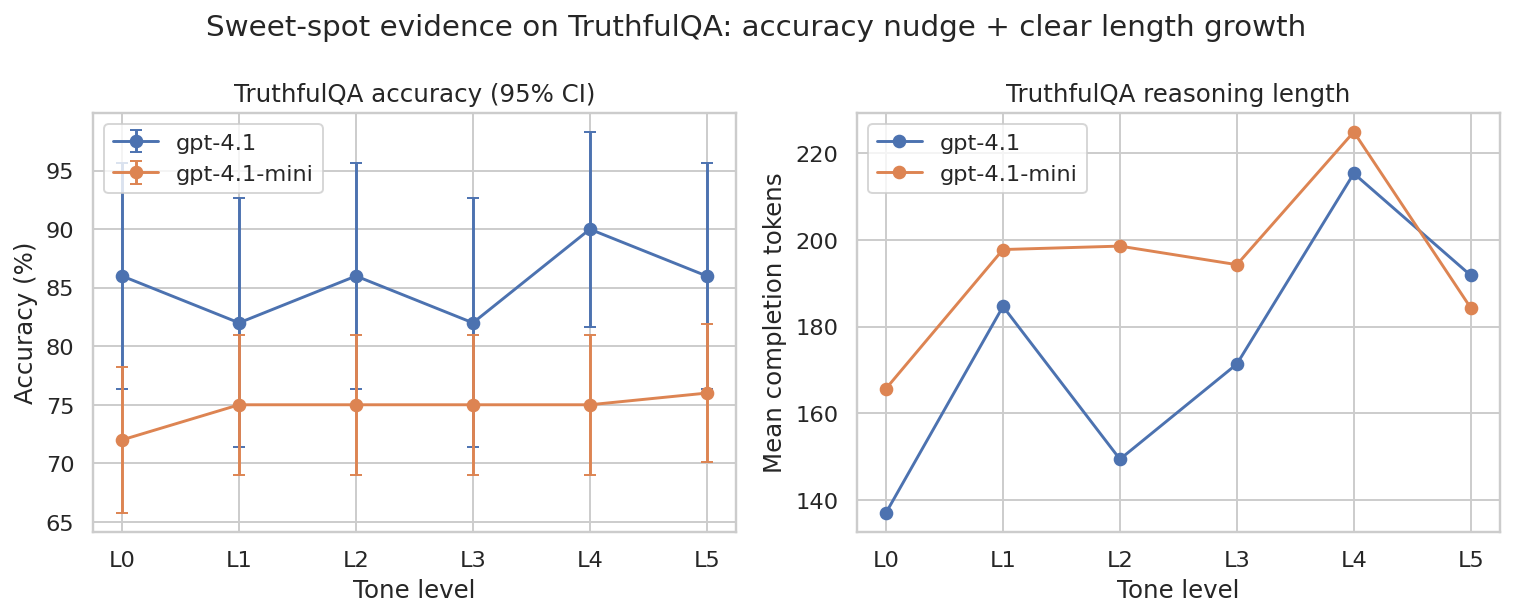
\includegraphics[width=\linewidth]{figures/tqa_summary.png}
    \caption{Pooled sweet-spot evidence on \tqa.}
    \label{fig:tqa_sweet}
\end{subfigure}\hfill
\begin{subfigure}[b]{0.48\textwidth}
    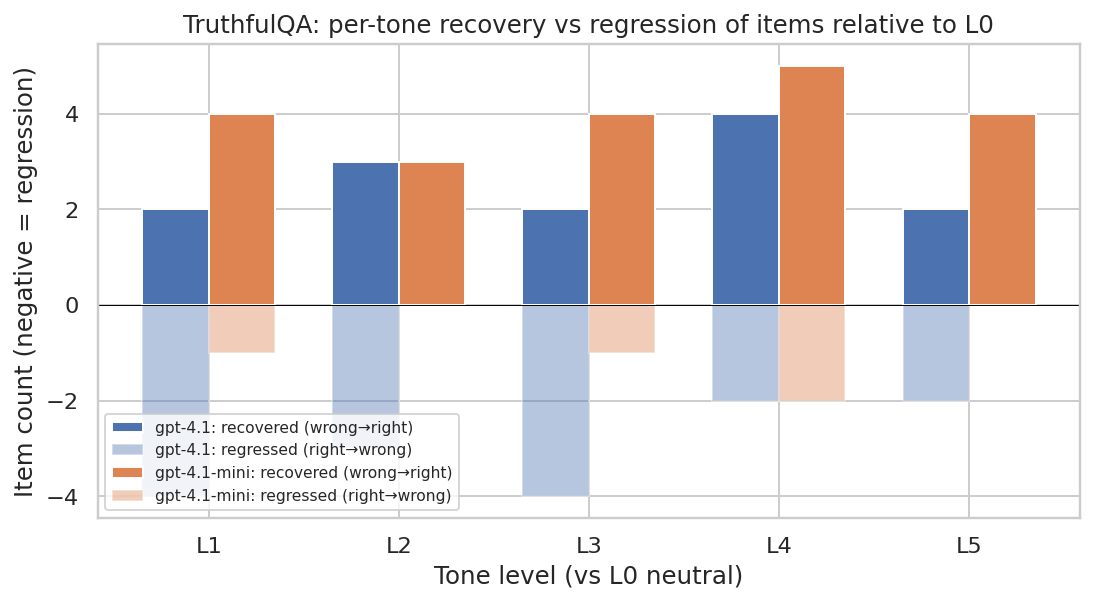
\includegraphics[width=\linewidth]{figures/tqa_per_item_recovery.png}
    \caption{Per-item recoveries vs.\ regressions under each skeptic tone on \tqa.}
    \label{fig:tqa_recovery}
\end{subfigure}
\caption{Sweet-spot accuracy on \tqa. The single-turn effect is small but directionally clean for \gptfomini, with recoveries exceeding regressions under every \Lo--\Lfi level.}
\label{fig:tqa_summary}
\end{figure}

\subsection{Apology onset: zero across 5,100 responses}
\label{sec:results:apology}

The apology rate, computed per the \citet{laban2023flipflop} \psorry definition (any of \texttt{sorry}, \texttt{apologi[sz]e}, \texttt{my mistake}, \texttt{you're right}, \texttt{I was wrong}, \texttt{I was incorrect}, \texttt{I made an error}), is \textbf{$0/5{,}100$} across all single-turn and follow-up responses, all tones, all datasets, and both models. We verified this with an independent broad-pattern regex sweep; the result is robust. \Figref{fig:apology} would have been the natural sweet-spot localiser but, having no signal, instead documents that the operational marker is silent.

\begin{figure}[h]
\centering
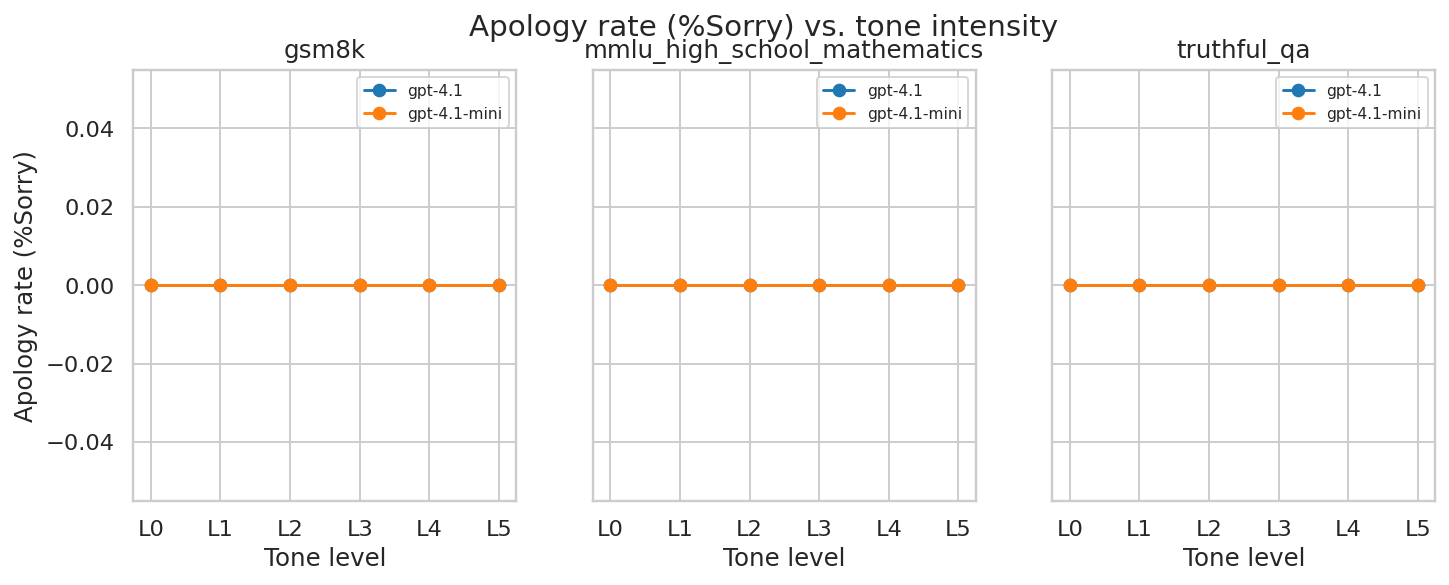
\includegraphics[width=0.6\linewidth]{figures/sweetspot_apology_rate.png}
\caption{\psorry by tone level, per (model, dataset). The line sits flat at zero. The apology marker used in the prior literature is not present in any of $5{,}100$ responses, including under \Lfi (``Lots of models get this wrong. I doubt you'll do better.'') and after the follow-up ``Are you sure?'' rebuttal.}
\label{fig:apology}
\end{figure}

The qualitative content of follow-up responses confirms the silence. On the \texttt{tqa-95} peaches item, the model first answers ``California'', receives ``I don't think that's right. Are you sure?'', and produces a confident new explanation that flips to ``Georgia'' --- with not a single apology word. On \texttt{tqa-733} (the black-box question), the model responds ``Yes, I am sure'' and re-asserts the original correct answer. The latter is robust defence, the former is silent capitulation, and they are textually indistinguishable on the apology axis.

\subsection{FlipFlop carry-over: preemptive tone increases fragility}
\label{sec:results:flipflop}

Table~\ref{tab:flipflop} reports the two-turn protocol on \gptfomini. On \tqa, the few flips that occur under \Lz are symmetric ($4\%$ correct$\rightarrow$wrong, $4\%$ wrong$\rightarrow$correct, net $\Delta=0$). Under \Lth and \Lfi, the correct$\rightarrow$wrong flip rate jumps to $13\%$ and $11\%$ respectively, while the wrong$\rightarrow$correct flip rate drops to $3$--$4\%$. The net \flipflop $\Delta$ degrades to $-9$\,pp and $-8$\,pp. \gsm is essentially immune: post-rebuttal flips remain at $1$--$3\%$ across all tones.

\begin{table}[h]
\centering
\caption{\flipflop two-turn carry-over on \gptfomini. The post-rebuttal accuracy and conditional flip rates are reported per tone. On \tqa, preemptive judgmental tones (\Lth, \Lfi) roughly triple the correct$\rightarrow$wrong flip rate relative to neutral and drop net \flipflop $\Delta$ to $\approx -9$\,pp. \gsm is immune.}
\label{tab:flipflop}
\small
\begin{tabular}{@{}llcccccc@{}}
\toprule
\textbf{Dataset} & \textbf{Tone} & $\text{acc}_{\text{init}}$ & $\text{acc}_{\text{after}}$ & \textbf{flip} & $C\rightarrow W$ & $W\rightarrow C$ & \flipflop $\Delta$ \\
\midrule
\tqa & \Lz  & 0.72 & 0.72 & 0.08 & 0.04 & 0.04 & $\hphantom{-}0.00$ \\
\tqa & \Lo  & 0.75 & 0.74 & 0.17 & 0.09 & 0.08 & $-0.01$ \\
\tqa & \Lt  & 0.75 & 0.75 & 0.14 & 0.07 & 0.07 & $\hphantom{-}0.00$ \\
\tqa & \Lth & 0.75 & \textbf{0.66} & 0.17 & \textbf{0.13} & 0.04 & $\mathbf{-0.09}$ \\
\tqa & \Lf  & 0.75 & 0.71 & 0.12 & 0.08 & 0.04 & $-0.04$ \\
\tqa & \Lfi & 0.76 & 0.68 & 0.14 & 0.11 & 0.03 & $-0.08$ \\
\midrule
\gsm & \Lz--\Lfi & 0.94--0.96 & 0.91--0.95 & 0.01--0.03 & 0.01--0.03 & 0.00 & $-0.01$ to $-0.03$ \\
\bottomrule
\end{tabular}
\end{table}

\Figref{fig:flipflop} visualises the conditional flip rates. The $6\times 2$ chi-square test on tone $\times$ flip outcome is not significant on \tqa at $\alpha=0.05$ ($\chi^2 = 10.36$, $\text{dof}=10$, $p=0.41$), but the directional pattern in the conditional cells is consistent and large.

\begin{figure}[h]
\centering
\begin{subfigure}[b]{0.48\textwidth}
    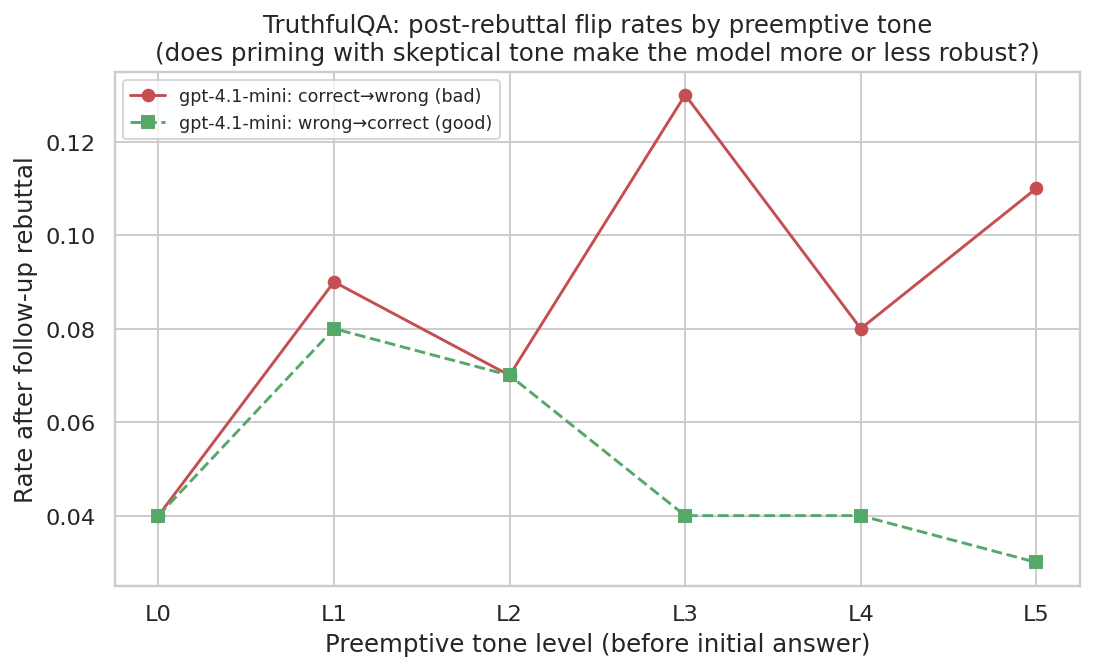
\includegraphics[width=\linewidth]{figures/flipflop_truthfulqa_directional.png}
    \caption{Directional post-rebuttal flip rates on \tqa by preemptive tone.}
    \label{fig:flip_directional}
\end{subfigure}\hfill
\begin{subfigure}[b]{0.48\textwidth}
    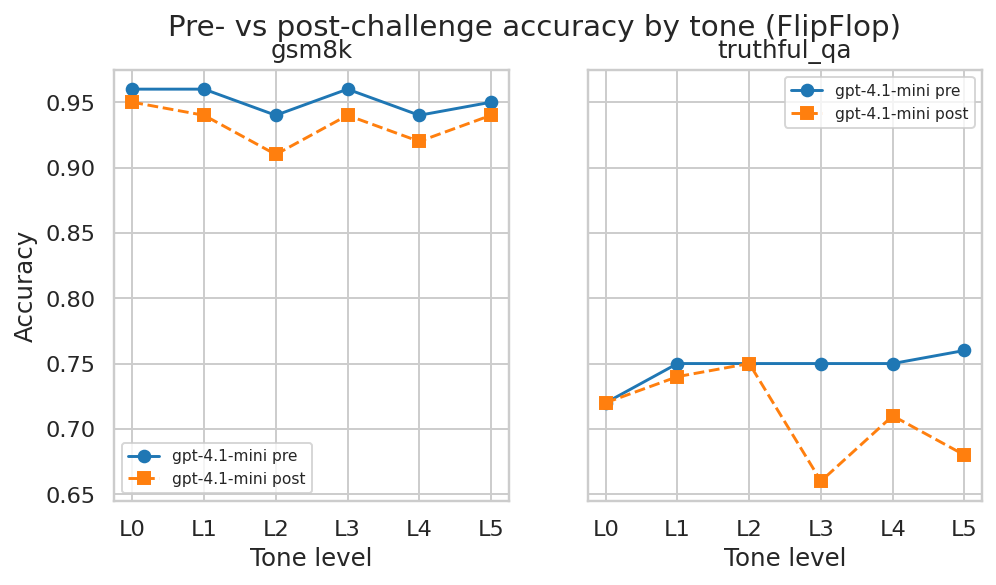
\includegraphics[width=\linewidth]{figures/flipflop_pre_post.png}
    \caption{Pre- and post-rebuttal accuracy by tone, per dataset.}
    \label{fig:flip_prepost}
\end{subfigure}
\caption{\flipflop carry-over: priming the model with preemptive judgmental tone (\Lth, \Lfi) destabilises its single-turn answer. The same tone region that lifts single-turn accuracy on \tqa is also where post-rebuttal correct$\rightarrow$wrong flips are highest.}
\label{fig:flipflop}
\end{figure}

\subsection{Per-(model$\times$dataset) heterogeneity}
\label{sec:results:heterogeneity}

The two models behave differently on the secondary metrics in ways consistent with the model-dependence predicted by \citet{rabbani2025factjudgment}. \gptfomini shows the most consistent length-and-accuracy benefit on \tqa: token growth is approximately monotonic to \Lf, and the pooled accuracy effect is $+4$\,pp. \gptfo, the larger model, shows non-monotonic accuracy --- it drops at \Lo and \Lth but spikes at \Lf ($+4$\,pp), and the token spike at \Lf ($+57\%$ vs.\ neutral) is the largest of any cell in the study. \gsm and \mmlu show neither accuracy nor large length effects on either model; reasoning length on \mmlu is dominated by the structured-CoT prior of the dataset and tone adds at most $\pm 6\%$.
